\documentclass{standalone}
\usepackage{tikz}
\usetikzlibrary{patterns, positioning}

\begin{document}
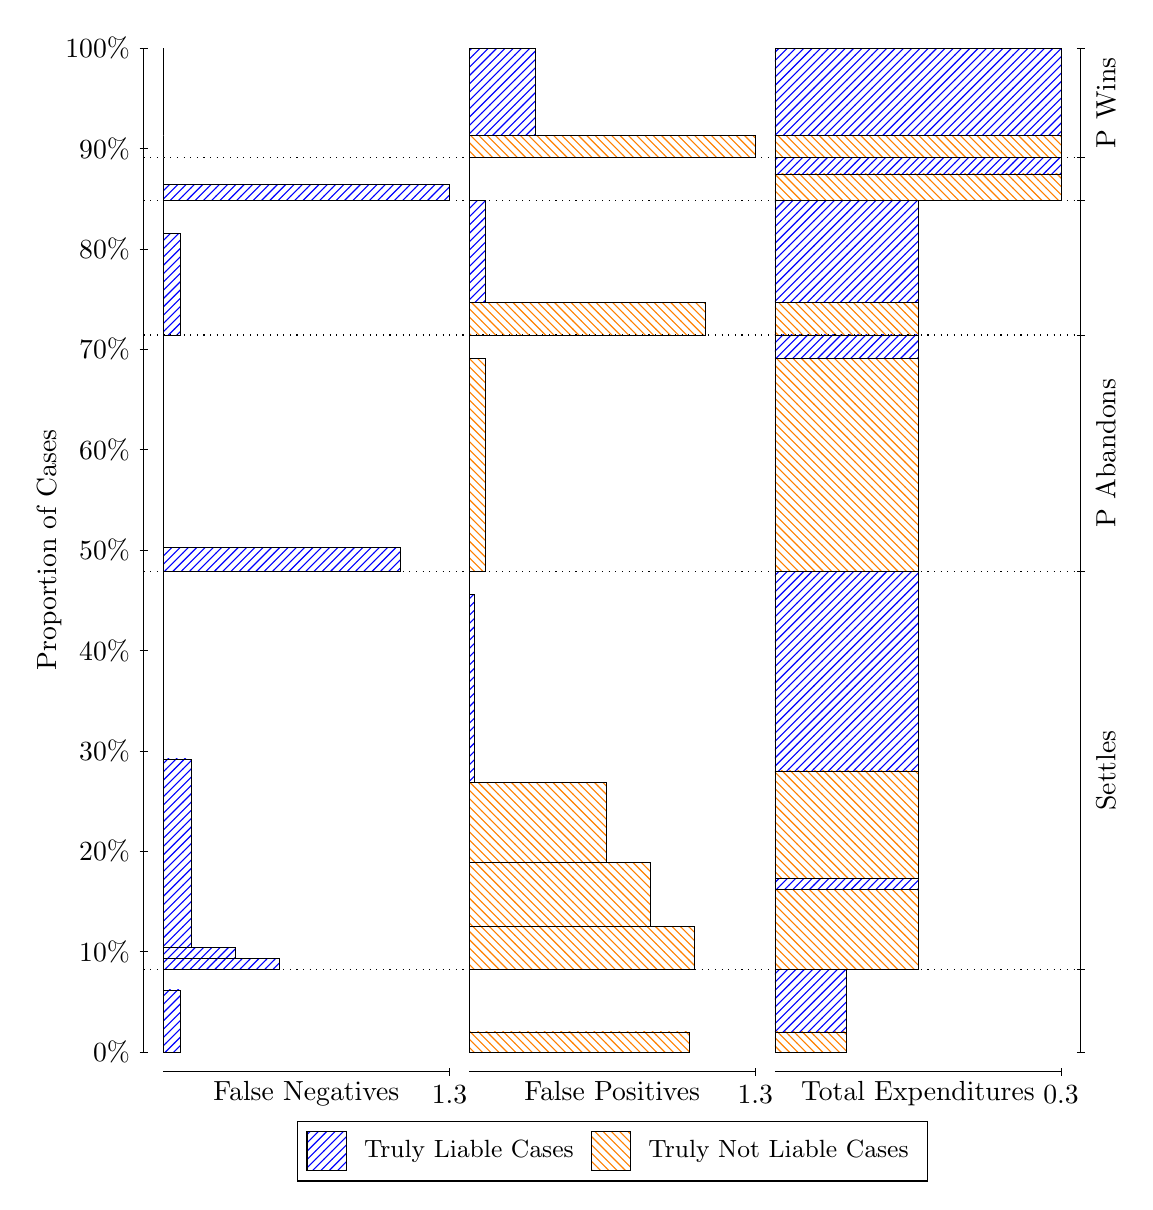
\begin{tikzpicture}
\draw[black, very thin] (1.5,1.75) -- (1.5,14.5);
\node[rotate=90, anchor=center] at (0.3, 8.125) {Proportion of Cases};
\draw[black, very thin] (1.45,1.75) -- (1.55,1.75);
\node[anchor=east] at (1.45, 1.75) {0\%};
\draw[black, very thin] (1.45,3.025) -- (1.55,3.025);
\node[anchor=east] at (1.45, 3.025) {10\%};
\draw[black, very thin] (1.45,4.3) -- (1.55,4.3);
\node[anchor=east] at (1.45, 4.3) {20\%};
\draw[black, very thin] (1.45,5.575) -- (1.55,5.575);
\node[anchor=east] at (1.45, 5.575) {30\%};
\draw[black, very thin] (1.45,6.85) -- (1.55,6.85);
\node[anchor=east] at (1.45, 6.85) {40\%};
\draw[black, very thin] (1.45,8.125) -- (1.55,8.125);
\node[anchor=east] at (1.45, 8.125) {50\%};
\draw[black, very thin] (1.45,9.4) -- (1.55,9.4);
\node[anchor=east] at (1.45, 9.4) {60\%};
\draw[black, very thin] (1.45,10.675) -- (1.55,10.675);
\node[anchor=east] at (1.45, 10.675) {70\%};
\draw[black, very thin] (1.45,11.95) -- (1.55,11.95);
\node[anchor=east] at (1.45, 11.95) {80\%};
\draw[black, very thin] (1.45,13.225) -- (1.55,13.225);
\node[anchor=east] at (1.45, 13.225) {90\%};
\draw[black, very thin] (1.45,14.5) -- (1.55,14.5);
\node[anchor=east] at (1.45, 14.5) {100\%};

\draw[black, very thin] (13.4,1.75) -- (13.4,14.5);
\draw[black, very thin] (13.35,1.75) -- (13.45,1.75);
\node[anchor=west] at (13.35, 1.75) {};
\draw[black, very thin] (13.35,2.7957) -- (13.45,2.7957);
\node[anchor=west] at (13.35, 2.7957) {};
\draw[black, very thin] (13.35,7.8523) -- (13.45,7.8523);
\node[anchor=west] at (13.35, 7.8523) {};
\draw[black, very thin] (13.35,10.856) -- (13.45,10.856);
\node[anchor=west] at (13.35, 10.856) {};
\draw[black, very thin] (13.35,12.564) -- (13.45,12.564);
\node[anchor=west] at (13.35, 12.564) {};
\draw[black, very thin] (13.35,13.109) -- (13.45,13.109);
\node[anchor=west] at (13.35, 13.109) {};
\draw[black, very thin] (13.35,14.5) -- (13.45,14.5);
\node[anchor=west] at (13.35, 14.5) {};

\draw[black, very thin, pattern color=blue, pattern=north east lines] (1.75,1.75) rectangle (1.9596,2.5393);
\draw[black, very thin, pattern color=orange, pattern=north west lines] (1.75,2.5393) rectangle (1.75,2.7957);
\draw[black, very thin, pattern color=blue, pattern=north east lines] (1.75,2.7957) rectangle (3.2173,2.9409);
\draw[black, very thin, pattern color=blue, pattern=north east lines] (1.75,2.9409) rectangle (2.6583,3.0825);
\draw[black, very thin, pattern color=blue, pattern=north east lines] (1.75,3.0825) rectangle (2.0994,5.4733);
\draw[black, very thin, pattern color=orange, pattern=north west lines] (1.75,5.4733) rectangle (1.75,7.8523);
\draw[black, very thin, pattern color=blue, pattern=north east lines] (1.75,7.8523) rectangle (4.7545,8.1547);
\draw[black, very thin, pattern color=orange, pattern=north west lines] (1.75,8.1547) rectangle (1.75,10.856);
\draw[black, very thin, pattern color=blue, pattern=north east lines] (1.75,10.856) rectangle (1.9596,12.146);
\draw[black, very thin, pattern color=orange, pattern=north west lines] (1.75,12.146) rectangle (1.75,12.564);
\draw[black, very thin, pattern color=blue, pattern=north east lines] (1.75,12.564) rectangle (5.3833,12.77);
\draw[black, very thin, pattern color=orange, pattern=north west lines] (1.75,12.77) rectangle (1.75,13.109);
\draw[black, very thin, pattern color=orange, pattern=north west lines] (1.75,13.109) rectangle (1.75,13.39);
\draw[black, very thin, pattern color=blue, pattern=north east lines] (1.75,13.39) rectangle (1.75,14.5);
\draw[black, very thin, pattern color=orange, pattern=north west lines] (5.6333,1.75) rectangle (8.4282,2.0064);
\draw[black, very thin, pattern color=blue, pattern=north east lines] (5.6333,2.0064) rectangle (5.6333,2.7957);
\draw[black, very thin, pattern color=orange, pattern=north west lines] (5.6333,2.7957) rectangle (8.4981,3.3477);
\draw[black, very thin, pattern color=orange, pattern=north west lines] (5.6333,3.3477) rectangle (7.9391,4.1579);
\draw[black, very thin, pattern color=orange, pattern=north west lines] (5.6333,4.1579) rectangle (7.3801,5.1747);
\draw[black, very thin, pattern color=blue, pattern=north east lines] (5.6333,5.1747) rectangle (5.7032,7.5655);
\draw[black, very thin, pattern color=blue, pattern=north east lines] (5.6333,7.5655) rectangle (5.6333,7.8523);
\draw[black, very thin, pattern color=orange, pattern=north west lines] (5.6333,7.8523) rectangle (5.8429,10.554);
\draw[black, very thin, pattern color=blue, pattern=north east lines] (5.6333,10.554) rectangle (5.6333,10.856);
\draw[black, very thin, pattern color=orange, pattern=north west lines] (5.6333,10.856) rectangle (8.6378,11.274);
\draw[black, very thin, pattern color=blue, pattern=north east lines] (5.6333,11.274) rectangle (5.8429,12.564);
\draw[black, very thin, pattern color=orange, pattern=north west lines] (5.6333,12.564) rectangle (5.6333,12.903);
\draw[black, very thin, pattern color=blue, pattern=north east lines] (5.6333,12.903) rectangle (5.6333,13.109);
\draw[black, very thin, pattern color=orange, pattern=north west lines] (5.6333,13.109) rectangle (9.2667,13.39);
\draw[black, very thin, pattern color=blue, pattern=north east lines] (5.6333,13.39) rectangle (6.4718,14.5);
\draw[black, very thin, pattern color=orange, pattern=north west lines] (9.5167,1.75) rectangle (10.425,2.0064);
\draw[black, very thin, pattern color=blue, pattern=north east lines] (9.5167,2.0064) rectangle (10.425,2.7957);
\draw[black, very thin, pattern color=orange, pattern=north west lines] (9.5167,2.7957) rectangle (11.333,3.8125);
\draw[black, very thin, pattern color=blue, pattern=north east lines] (9.5167,3.8125) rectangle (11.333,3.9577);
\draw[black, very thin, pattern color=orange, pattern=north west lines] (9.5167,3.9577) rectangle (11.333,5.3199);
\draw[black, very thin, pattern color=blue, pattern=north east lines] (9.5167,5.3199) rectangle (11.333,7.8523);
\draw[black, very thin, pattern color=orange, pattern=north west lines] (9.5167,7.8523) rectangle (11.333,10.554);
\draw[black, very thin, pattern color=blue, pattern=north east lines] (9.5167,10.554) rectangle (11.333,10.856);
\draw[black, very thin, pattern color=orange, pattern=north west lines] (9.5167,10.856) rectangle (11.333,11.274);
\draw[black, very thin, pattern color=blue, pattern=north east lines] (9.5167,11.274) rectangle (11.333,12.564);
\draw[black, very thin, pattern color=orange, pattern=north west lines] (9.5167,12.564) rectangle (13.15,12.903);
\draw[black, very thin, pattern color=blue, pattern=north east lines] (9.5167,12.903) rectangle (13.15,13.109);
\draw[black, very thin, pattern color=orange, pattern=north west lines] (9.5167,13.109) rectangle (13.15,13.39);
\draw[black, very thin, pattern color=blue, pattern=north east lines] (9.5167,13.39) rectangle (13.15,14.5);
\draw[black, dotted] (1.5,2.7957) -- (13.4,2.7957);
\draw[black, dotted] (1.5,7.8523) -- (13.4,7.8523);
\draw[black, dotted] (1.5,10.856) -- (13.4,10.856);
\draw[black, dotted] (1.5,12.564) -- (13.4,12.564);
\draw[black, dotted] (1.5,13.109) -- (13.4,13.109);
\draw[black, very thin] (1.75,1.5) -- (5.3833,1.5);
\node[anchor=north] at (3.5667, 1.5) {False Negatives};
\draw[black, very thin] (5.3833,1.45) -- (5.3833,1.55);
\node[anchor=north] at (5.3833, 1.45) {1.3};

\draw[black, very thin] (5.6333,1.5) -- (9.2667,1.5);
\node[anchor=north] at (7.45, 1.5) {False Positives};
\draw[black, very thin] (9.2667,1.45) -- (9.2667,1.55);
\node[anchor=north] at (9.2667, 1.45) {1.3};

\draw[black, very thin] (9.5167,1.5) -- (13.15,1.5);
\node[anchor=north] at (11.333, 1.5) {Total Expenditures};
\draw[black, very thin] (13.15,1.45) -- (13.15,1.55);
\node[anchor=north] at (13.15, 1.45) {0.3};


\node[black, centered, rotate=90] at (13.72, 5.324) {Settles};
\node[black, centered, rotate=90] at (13.72, 9.3544) {P Abandons};


\node[black, centered, rotate=90] at (13.72, 13.805) {P Wins};

\draw (7.449999999999999,1.5) node[draw=none] (baseCoordinate) {};
\begin{scope}[align=center]
        \matrix[scale=0.5, draw=black, below=0.5cm of baseCoordinate, nodes={draw}, column sep=0.1cm]{
            \node[rectangle, draw, minimum width=0.5cm, minimum height=0.5cm, pattern=north east lines, pattern color=blue] {}; &
            \node[draw=none, font=\small] (B) {Truly Liable Cases}; &
            \node[rectangle, draw, minimum width=0.5cm, minimum height=0.5cm, pattern=north west lines, pattern color=orange] {}; &
            \node[draw=none, font=\small] (B) {Truly Not Liable Cases}; \\
            };
\end{scope}

\end{tikzpicture}
\end{document}